\begin{frame}{Bulk Entanglement and Edges}
%We can (heuristically for now) connect the existence of the edge state to the idea that these types of insulators are really distinct from atomic insulators. 
\vskip-1.5cm
Bulk ground state contains information about edge physics
\bi
\item  Imagine cutting IQH state in half, forming edge states $\ket{k}_{L, R}$
%or another state with a protected edge
%at this point, the eigenstates of the system are factored between left and right sides
% the lowest energy states look like ground states far away, but differ at the edge due to the edge modes 
\item Adiabatically tune the coupling back to normal value 
%and find the new ground state
\item System can lower its energy by coupling the currents
\item Entangled eigenstate $\sum \ket{k}_L \otimes\ket{-k}_R$ 
% But this is just the regular state of the system with no cut at all!
\item Atomic insulator wavefunctions factor trivially - no entanglement.
% This suggests that these are distinct phases of matter from atomic insulators, we should look at entanglement and show that the entanglement is robust to perturbations. This can be a route to showing the edge is robust to (certain) perturbations without having to worry about the actual precise form of the edge.  
\ei 
\vskip-0.2cm
\begin{figure}
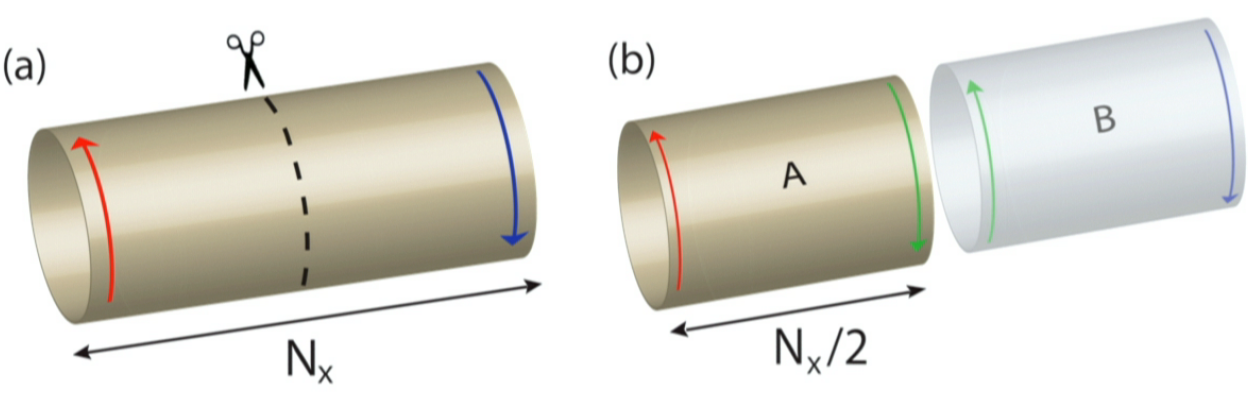
\includegraphics[width=\linewidth]{diagrams/entanglement_cut.png}
\end{figure}
\footnotetext[3]{
\citep{Alexandradinata2011-os}} 
\end{frame}

